%%% LaTeX Template
%%% This template is made for project reports
%%%	You may adjust it to your own needs/purposes
%%%
%%% Copyright: http://www.howtotex.com/
%%% Date: March 2011

%%% Preamble
\documentclass[paper=a4, fontsize=11pt]{scrartcl}	% Article class of KOMA-script with 11pt font and a4 format
\usepackage[OT4]{fontenc}
\usepackage[utf8]{inputenc}
\usepackage{fourier}

\usepackage[polish]{babel}															% English language/hyphenation
\usepackage[protrusion=true,expansion=true]{microtype}				% Better typography
\usepackage{amsmath,amsfonts,amsthm}										% Math packages
\usepackage[pdftex]{graphicx}														% Enable pdflatex
\usepackage{url}
\usepackage{mathtools}
\DeclarePairedDelimiter{\ceil}{\lceil}{\rceil}
\usepackage{multirow}
\usepackage[justification=centering]{caption} 

%%% Custom sectioning (sectsty package)
\usepackage{sectsty}												% Custom sectioning (see below)
\allsectionsfont{\centering \normalfont\scshape}	% Change font of al section commands


%%% Custom headers/footers (fancyhdr package)
\usepackage{fancyhdr}
\pagestyle{fancyplain}
\fancyhead{}														% No page header
\fancyfoot[C]{}													% Empty
\fancyfoot[R]{\thepage}									% Pagenumbering
\renewcommand{\headrulewidth}{0pt}			% Remove header underlines
\renewcommand{\footrulewidth}{0pt}				% Remove footer underlines
\setlength{\headheight}{13.6pt}
\addtolength{\topmargin}{-0.375in}
\textheight=24cm


%%% Equation and float numbering
\numberwithin{equation}{section}		% Equationnumbering: section.eq#
\numberwithin{figure}{section}			% Figurenumbering: section.fig#
\numberwithin{table}{section}				% Tablenumbering: section.tab#


%%% Maketitle metadata
\newcommand{\horrule}[1]{\rule{\linewidth}{#1}} 	% Horizontal rule

\title{
	%\vspace{-1in} 	
	\usefont{OT1}{bch}{b}{n}
	\normalfont \normalsize \textsc{Programowanie Współbieżne i Rozproszone 2013} \\ [25pt]
	\horrule{0.5pt} \\[0.4cm]
	\huge Raport: zadanie zaliczeniowe z MPI \\
	\horrule{2pt} \\[0.5cm]
}
\author{
	\normalfont \normalsize
        Wojciech Żółtak (292583) \\[-3pt] \normalsize
        \today
}
\date{}


\begin{document}
%%% Begin document

\maketitle

\section{Wstęp}
Niniejszy dokument zawiera opis rozwiązania zadania zaliczeniowego z MPI oraz
jego ewaluacji na klastrze obliczeniowym Halo2 w ICM.


\section{Rozwiązanie}

\subsection{Cechy problemu}
Celem ćwiczenia było zrównoleglenie gotowego programu wykonującego wiele
iteracji obliczeń w sekwencyjny sposób, z zachowaniem użytego algorytmu
numerycznego.\\

Posiada on następujące cechy:
\begin{itemize}
  \item{Obliczenia odbywają się na kwadratowej siatce $NxN$.}
  \item{Każda iteracja ma dwie fazy.}
  \item{Każda faza polega na wyliczeniu nowej wartości dla połowy punktów z
        siatki.}
  \item{Wartość w każdym punkcie zależy tylko od wartości punktów sąsiednich.}
  \item{Wykonanie kolejnej iteracji zależy od największej różnicy między starą a
        nową wartością w punktach siatki.}
\end{itemize}

Wynika z nich, że:
\begin{itemize}
  \item{Rozproszenie może polegać właściwie tylko na podziale obszaru siatki
        między węzły robocze.}
  \item{Synchronizacja węzłów musi następować co najmniej przed każdą z faz
        iteracji oraz po jej wykonaniu.}
\end{itemize}


\subsection{Opis rozwiązania}

Rozwiązanie opiera się na podziale obszaru roboczego na pasy szerokości
$\ceil{N / P}$, gdzie $N$ to długość boku siatki, a $P$ ilość procesów biorących
udział w obliczeniu. Pasy zostają przydzielone po jednym na proces, począwszy od
procesu z rangą 0. Procesy, ktorym nie starczy pasów nie pracują.\\

Dane generowane są przez proces o randze 0, a następnie rozsyłane do
odpowiednich węzłów w wiadomościach nie większych niż 1GB. Przesyłanie większych
wiadomości powodowało błędy infrastruktury Infiniband używanej w klastrze.\\

Ponieważ obliczenia wymagają wartości z sąsiednich punktów, zachodzi potrzeba
synchronizacji części danych pomiędzy procesami przed każdą z faz iteracji.
Wystarczy jednak przesłać jedynie dolną/górną krawędź pasa do ,,sąsiednich''
procesów. Odbywa się to przy pomocy asynchronicznej komendy
,,$\texttt{MPI\_Isend}$''.\\

\begin{figure}[h]
  \centering
    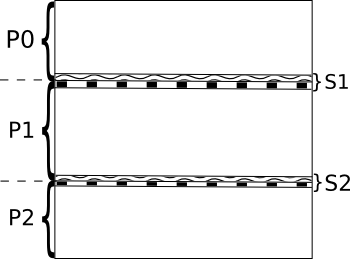
\includegraphics{report/podzial.png}
  \caption{Podział obszaru roboczego między trzy procesy P1, P2 i P3 wraz z
           dwoma synchronizowanymi obszarami S1 i S2 na krawędziach sąsiednich
           pasów.}
\end{figure}

Po zakończeniu iteracji procesy dokonują redukcji obliczonych różnic wartości za
pomocą funkcji minimum, a następnie sprawdzają czy należy kontynuować
obliczenia.\\

Wynik obliczeń jest agregowany i wypisywany przez proces o randze zero,
zbierający dane od pozostałych węzłów.



\section{Ewaluacja}

\subsection{Wykonane testy}

Parametry wykonanych testów ilustruje poniższa tabela:

\begin{figure}[h]
  \centering
  \begin{tabular}{|r|c|c|}
    \hline
     & $\texttt{laplace-seq}$ & $\texttt{laplace-par}$ \\
    \hline
    \multirow{2}{*}{Rozmiar boku siatki} &
	\multicolumn{2}{|c|}{2500, 5000, 10000, 15000,} \\
     & \multicolumn{2}{|c|}{20000, 25000, 30000, 40000} \\
    \hline
    \multirow{3}{*}{Zasoby} & \multirow{3}{*}{1-1} &
       1-1, 1-2, 2-1, 1-4, 4-1, \\
     &  & 1-8, 8-1, 16-1, 1-16, 2-2,  \\
     &  & 2-4, 4-2, 4-8, 8-4, 8-16, 16-8  \\
    \hline
  \end{tabular}
  \caption{Rozmiary siatki oraz przydzielone zasoby dla programów podczas
           testów. \newline Notacja ,,X-Y'' oznacza X maszyn po Y rdzeni.}
\end{figure}

Z powodu dużego obciążenia klastra wszystkie poza jednym
($\texttt{laplace-par-10000-4-2}$; użyty do sprawdzenia wariancji czasów)
zostały wykonane jednokrotnie.


\subsection{Program sekwencyjny}

Poniższy wykres ukazuje czas działania programu sekwencyjnego dla różnych
rozmiarów siatki:
\begin{figure}[h]
  \centering
    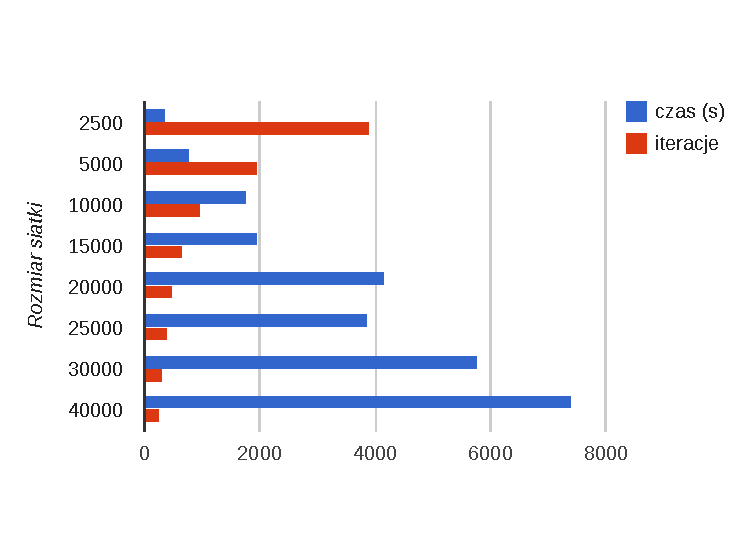
\includegraphics{report/seq-time.pdf}
  \caption{Czas działania oraz ilość iteracji wersji sekwencyjnej.}
\end{figure}

Widać dość wyraźne zaburzenie dla ${N=25000}$, który wydaje się działać szybciej
niż ${N=20000}$. Warto jednak zauważyć, że ilość iteracji spada wraz ze wzrostem
$N$, a zatem łączny czas sam w sobie nie pozwala na miarodajne porównywanie
wyników. To co nas interesuje to średni czas na iterację. Przyjrzyjmy się mu,
najlepiej od razu porównwując z wersją współbieżną w konfiguracji 1-1.

\begin{figure}[h]
  \centering
    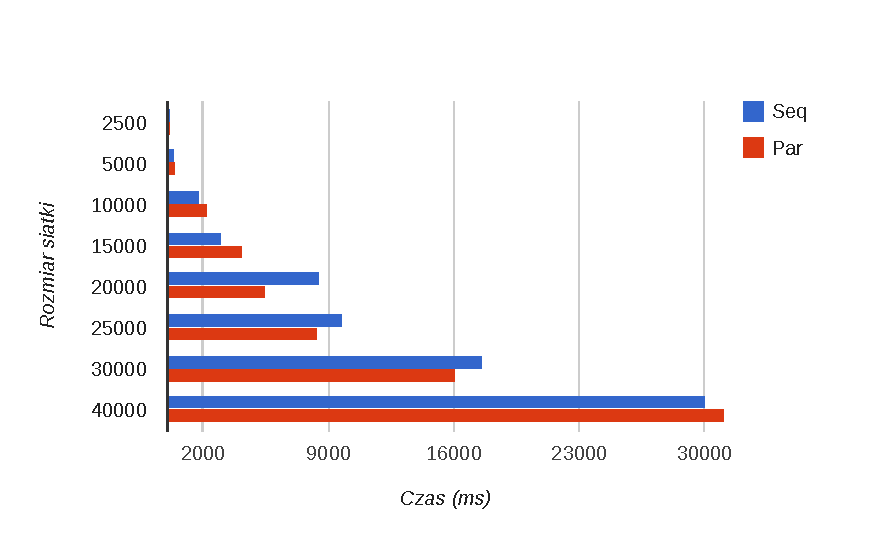
\includegraphics{report/seq-time-norm.pdf}
  \caption{Średni czas zużyty na iterację przez wersję sekwencyjną\newline
           i współbieżną w konfiguracji 1-1.}
\end{figure}

Wygląda to bardzo podobnie, ale nieco lepiej - teraz ${N=25000}$ jest
nieznacznie wolniejsze od ${N=20000}$. Niemniej, wydaje się, że test dla
${N=25000}$ działał w lepszych warunkach. Może węzeł na którym był liczony był
mniej obciążony? Ponadto, rozwiązanie współbieżne czasem jest szybsze, a czasem
wolniejsze, chociaż od strony kodu w zasadzie jest tym samym (posiada mały
narzut potrzebny na sprawdzenie, że nie musi się z nikim komunikować). \\

To prowadzi do pytania o powtarzalność testów.



\subsection{Test ,,wariancji''}

W celu sprawdzenia powtarzalności wyników uruchomiono test
,,${\texttt{par-10000-4-2}}$'' ośmiokrotnie.

%\begin{figure}[h]
%  \centering
\begin{center}
    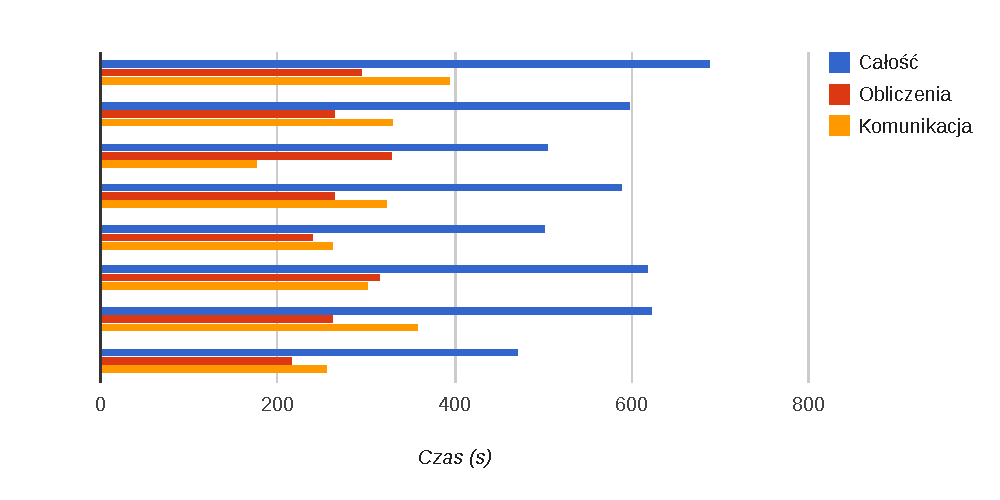
\includegraphics{report/var.pdf}
\end{center}
%  \caption{Czas zużyty przez kolejne wywołania testu
%     ,,$\texttt{par-10000-4-2}$''.}
%  \label{fig:varChart}
%\end{figure}

Jak widać na wykresie, czas wykonania bardzo się waha.
Różnica między najszybszym a najwolniejszym testem wynosi 216s! Co więcej,
zarówno czas obliczeń jak i zużyty na przesyłanie wiadomości wahają się, co każe
wnioskować, że nie jest to wina infrastruktury komunikacyjnej, lecz faktyczna
różnica w dostępnych zasobach CPU. \\

Prowadzi to do konkluzji, że jednokrotne wykonanie testów może dawać wyniki,
które nie są w pełni porównywalne. Jednakże, w obliczu przeciążonego klastra nie
pozostaje nam nic innego jak posiłkować się danymi, które zdołało się
wygenerować.


\subsection{Program współbieżny}

\subsubsection{Całkowity czas pracy}
Poniższe wykresy prezentują uśredniony czas iteracji dla różnych konfiguracji w
rozwiązaniu współbieżnym. Skala jest logarytmiczna. Ilość iteracji została
pominięta, gdyż jest dokładnie taka sama jak w rozwiązaniu sekwencyjnym.\\

Zauważyć można dwie rzeczy. \\

Po pierwsze, czas spada mniej więcej proporcjonalnie do wzrostu ilości procesów,
co świadczy o w miarę dobrym zrównolegleniu problemu. \\

Po drugie - konfiguracje
pracujące na mniejszej ilości maszyn, lecz większej ilości rdzeni mają przewagę
nad konfiguracjami odwrotnymi. Wynika to najprawdopodobniej z większej
lokalności w komunikacji, która rzadziej musi korzystać z łącz sieciowych.
Przewaga ta rośnie wraz z ilością danych, które muszą wymienić ze sobą procesy.
\\

\begin{center}

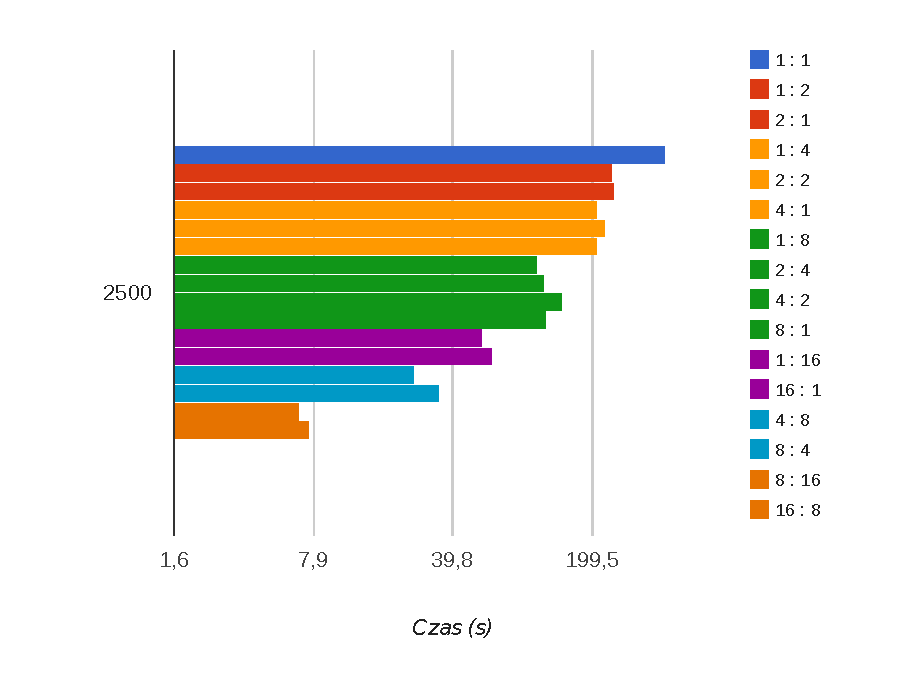
\includegraphics[width=135mm]{report/time-2500.pdf}

Różne konfiguracje współbieżne przy siatce o boku 2500.
\\ \ \\ \ \\


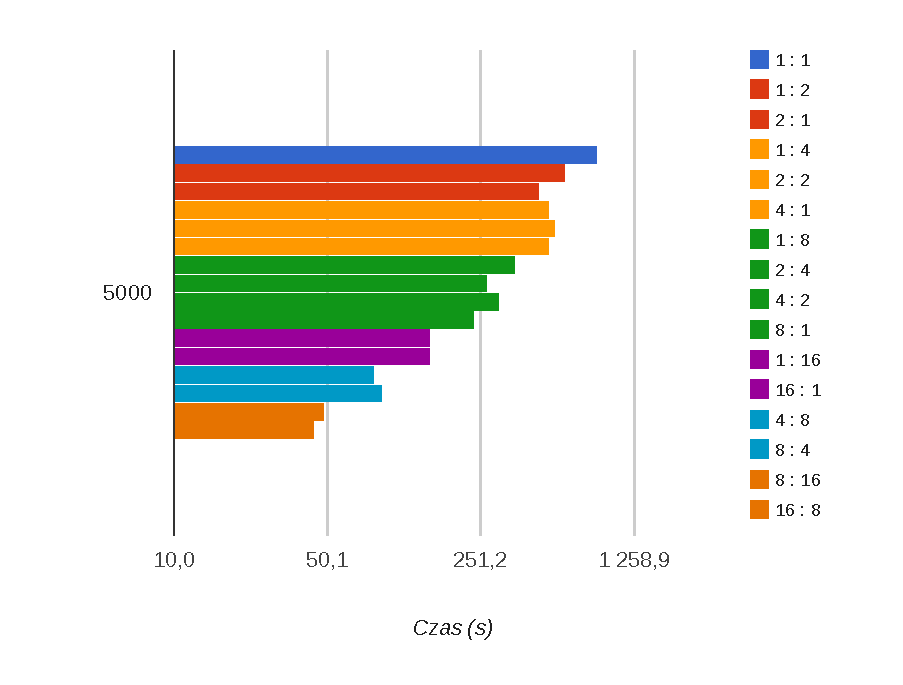
\includegraphics[width=135mm]{report/time-5000.pdf}

Różne konfiguracje współbieżne przy siatce o boku 5000.
\\ \ \\ \ \\


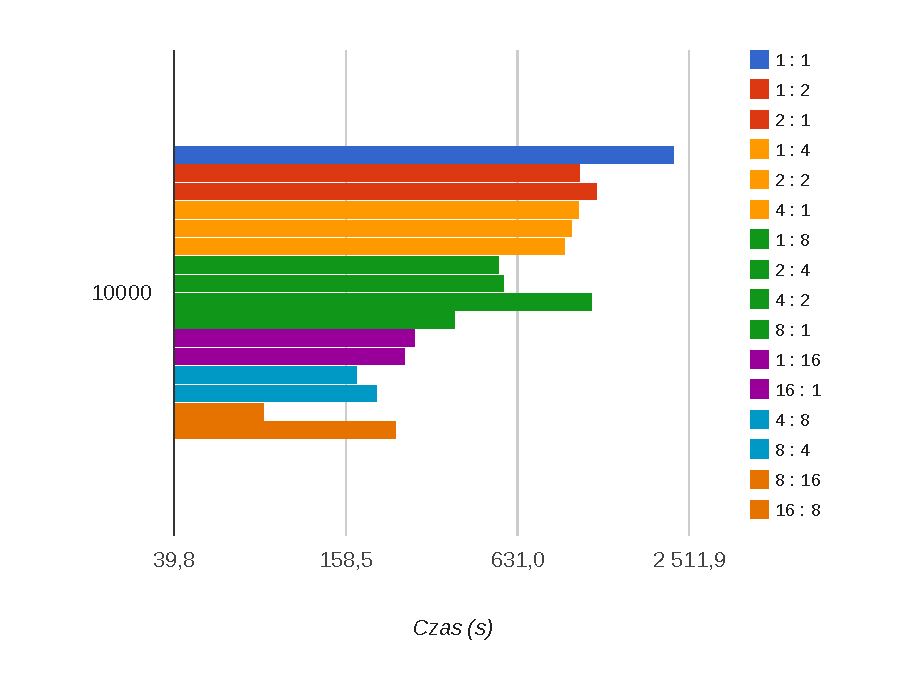
\includegraphics[width=135mm]{report/time-10000.pdf}

Różne konfiguracje współbieżne przy siatce o boku 10000.
\\ \ \\ \ \\


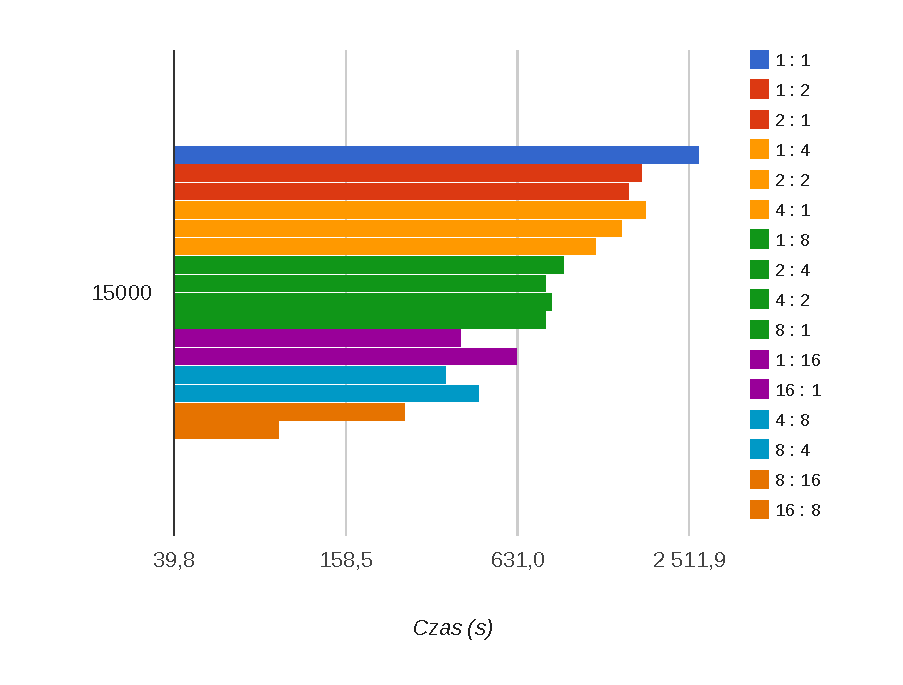
\includegraphics[width=135mm]{report/time-15000.pdf}

Różne konfiguracje współbieżne przy siatce o boku 15000.
\\ \ \\ \ \\


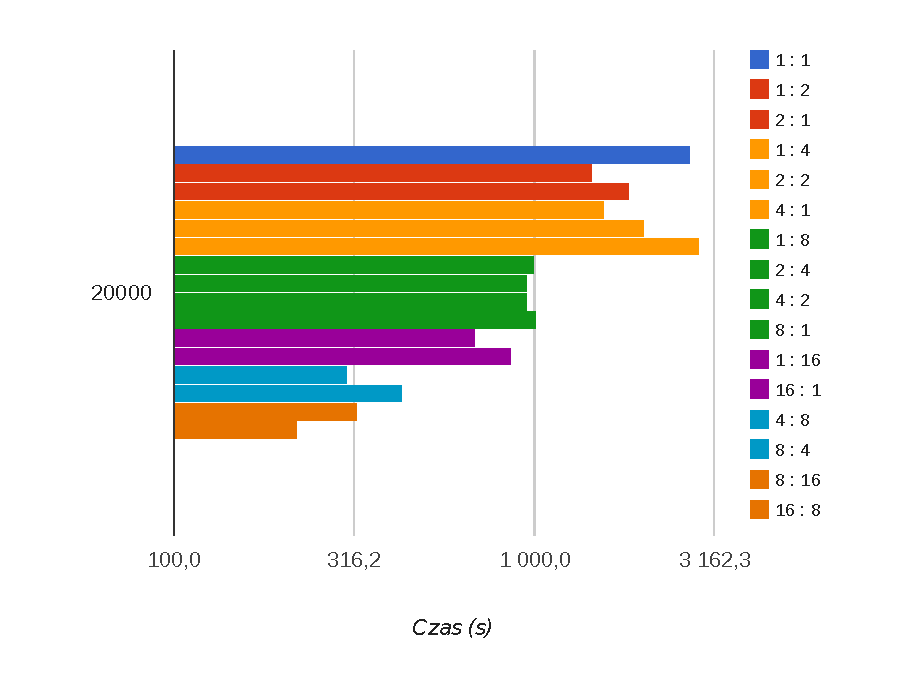
\includegraphics[width=135mm]{report/time-20000.pdf}

Różne konfiguracje współbieżne przy siatce o boku 20000.
\\ \ \\ \ \\


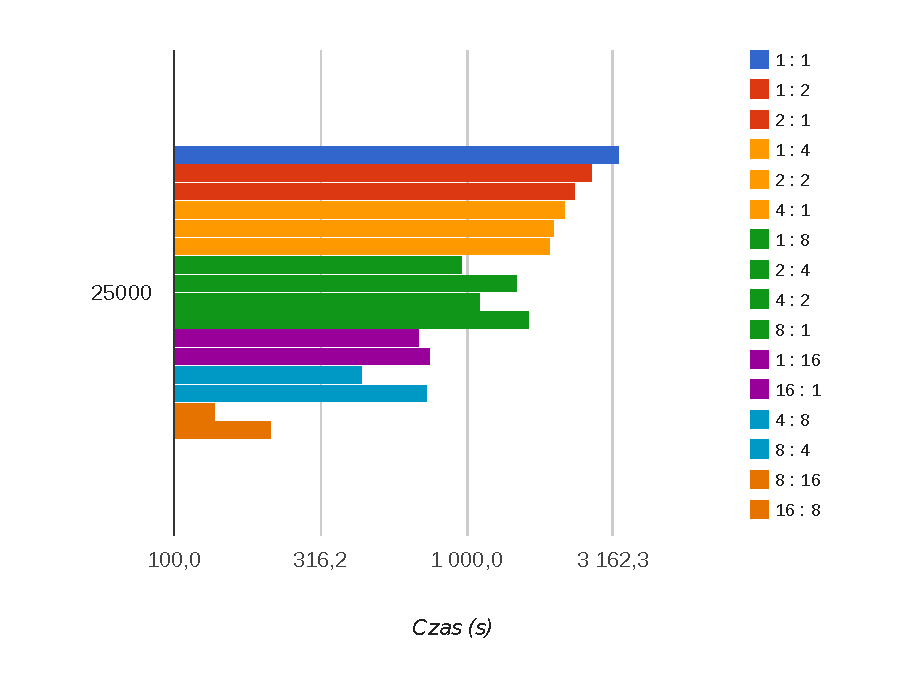
\includegraphics[width=135mm]{report/time-25000.pdf}

Różne konfiguracje współbieżne przy siatce o boku 25000.
\\ \ \\ \ \\


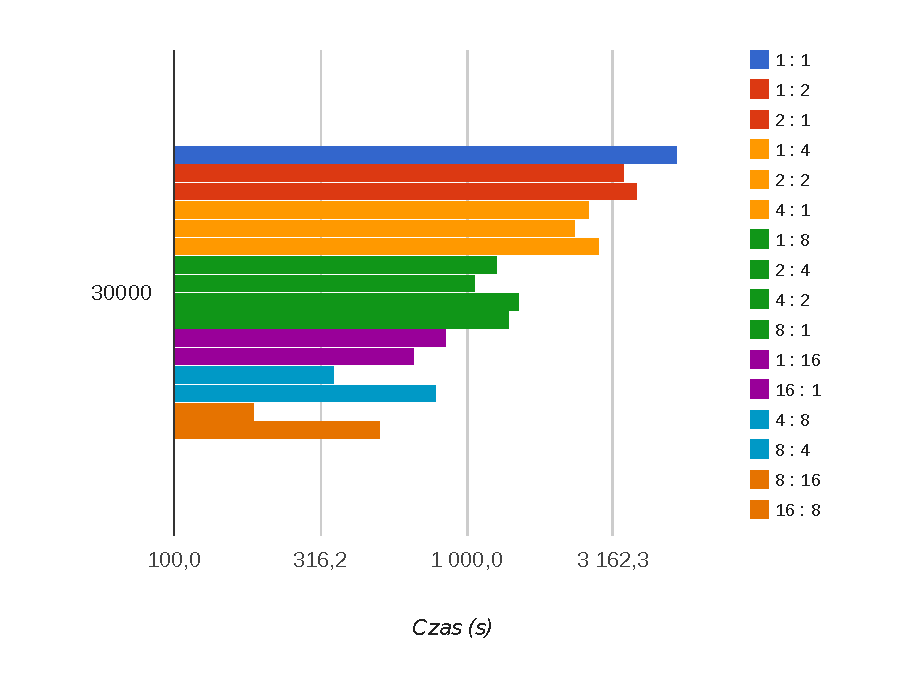
\includegraphics[width=135mm]{report/time-30000.pdf}

Różne konfiguracje współbieżne przy siatce o boku 30000.
\\ \ \\ \ \\


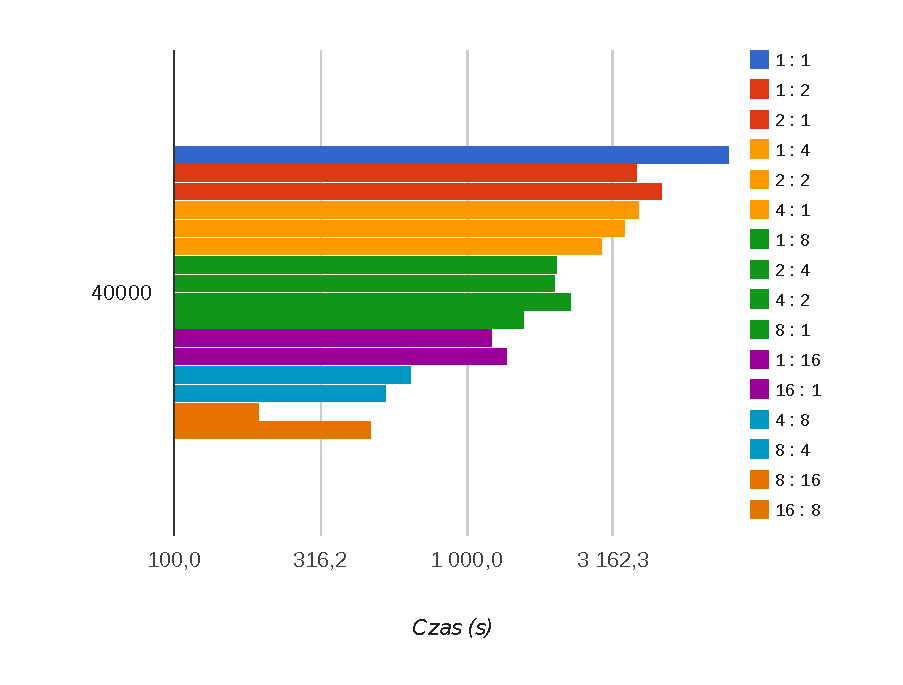
\includegraphics[width=135mm]{report/time-40000.pdf}

Różne konfiguracje współbieżne przy siatce o boku 40000.
\\ \ \\ \ \\

\end{center}


\subsubsection{Speedup całkowitego czasu wykonania}

Przyspieszenie całkowite liczone jest jako stosunek czasu wykonania programu
sekwencyjnego oraz współbieżnego. Liczby w nawiasach zamieszczone w legendzie to
łączna ilość procesów biorąca udział w teście. Testy o tej samej liczności
posiadają ten sam kolor słupków. \\

Wyraźnie widać, że przyspieszenie jest dalekie od ideału (będzie to lepiej widać
potem, na wykresach efektywności). Ponownie widać spore wahania wyników oraz
przewagę konfiguracji wielordzeniowych nad wielomaszynowymi.

\begin{center}

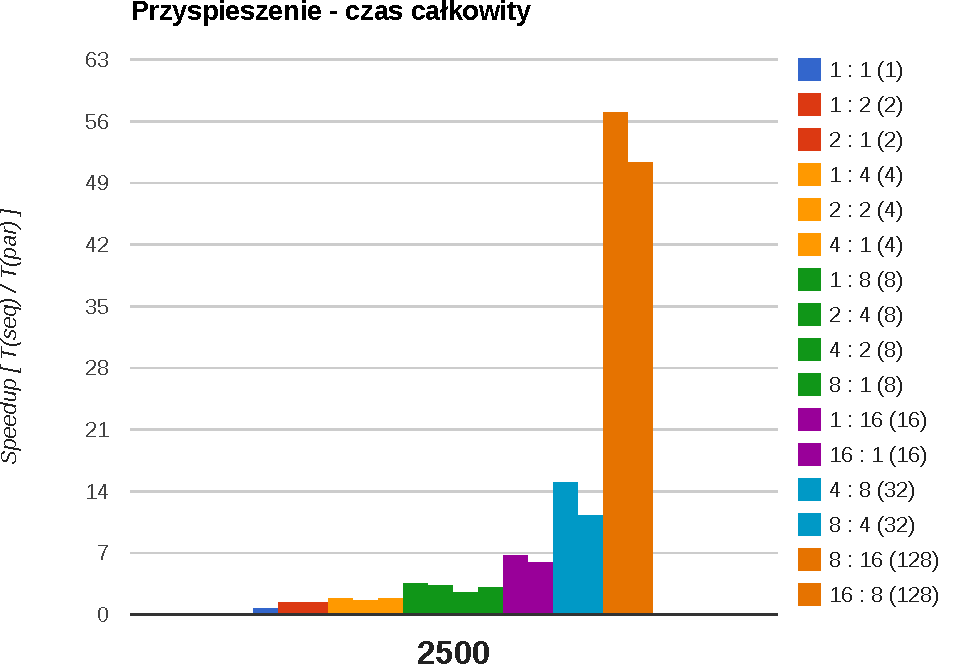
\includegraphics[width=135mm]{report/speedup-2500.pdf} \\ \ \\ \ \\ \ \\

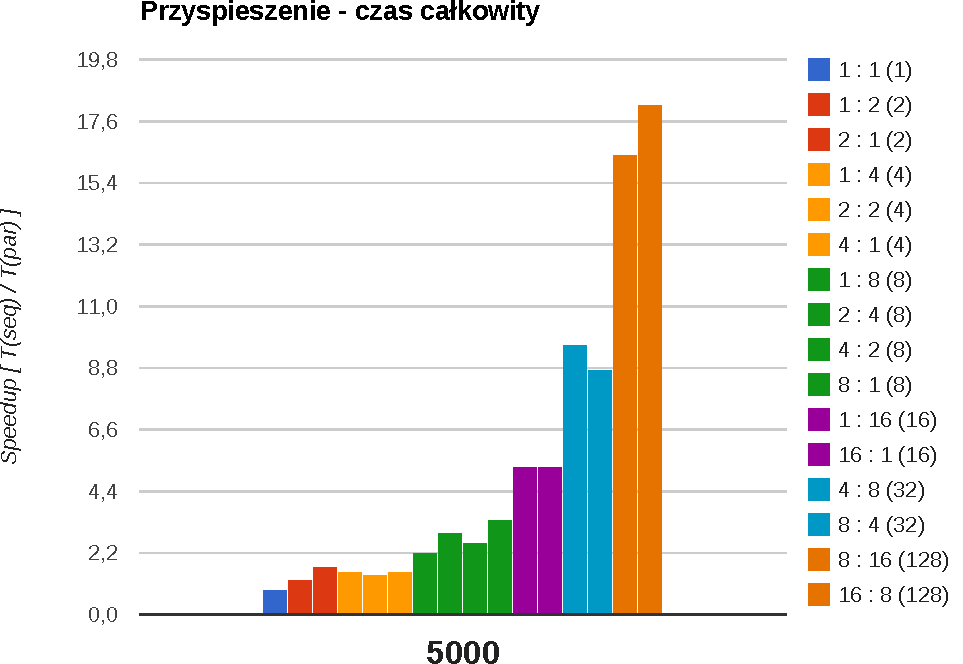
\includegraphics[width=135mm]{report/speedup-5000.pdf} \\ \ \\ \ \\ \ \\

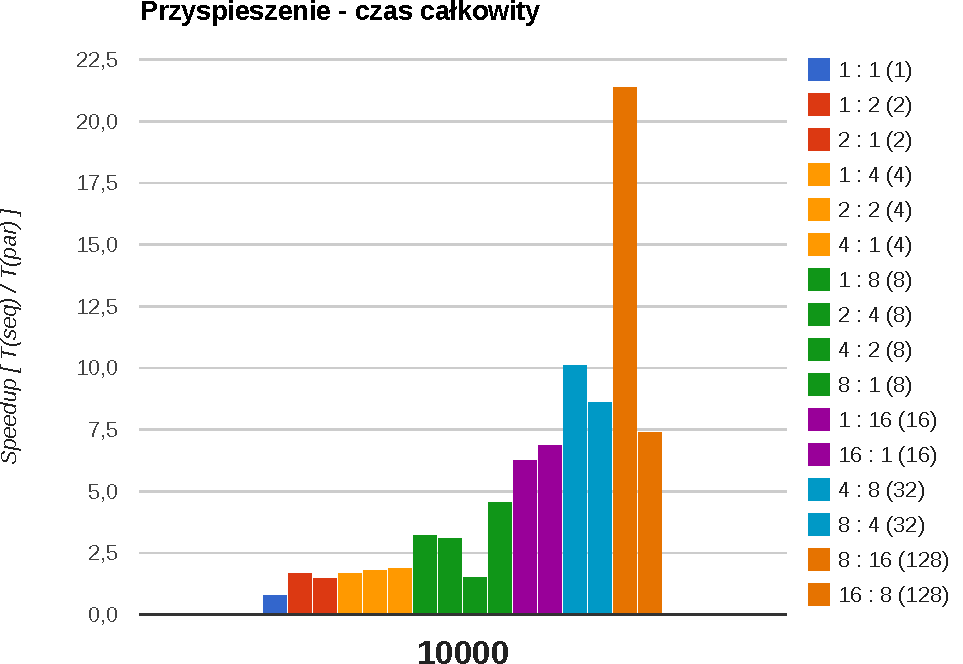
\includegraphics[width=135mm]{report/speedup-10000.pdf} \\ \ \\ \ \\ \ \\

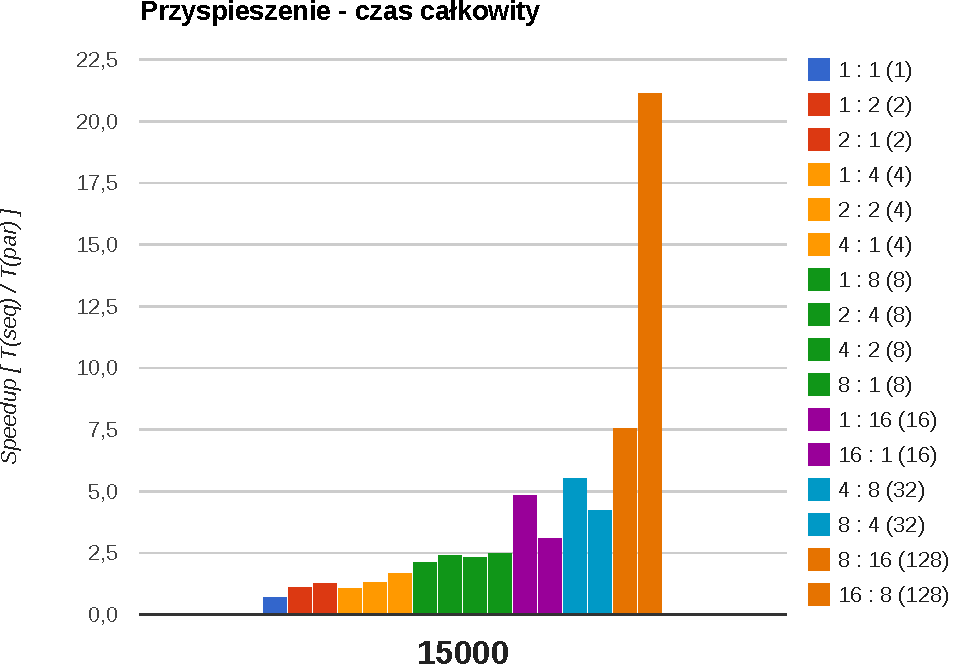
\includegraphics[width=135mm]{report/speedup-15000.pdf} \\ \ \\ \ \\ \ \\

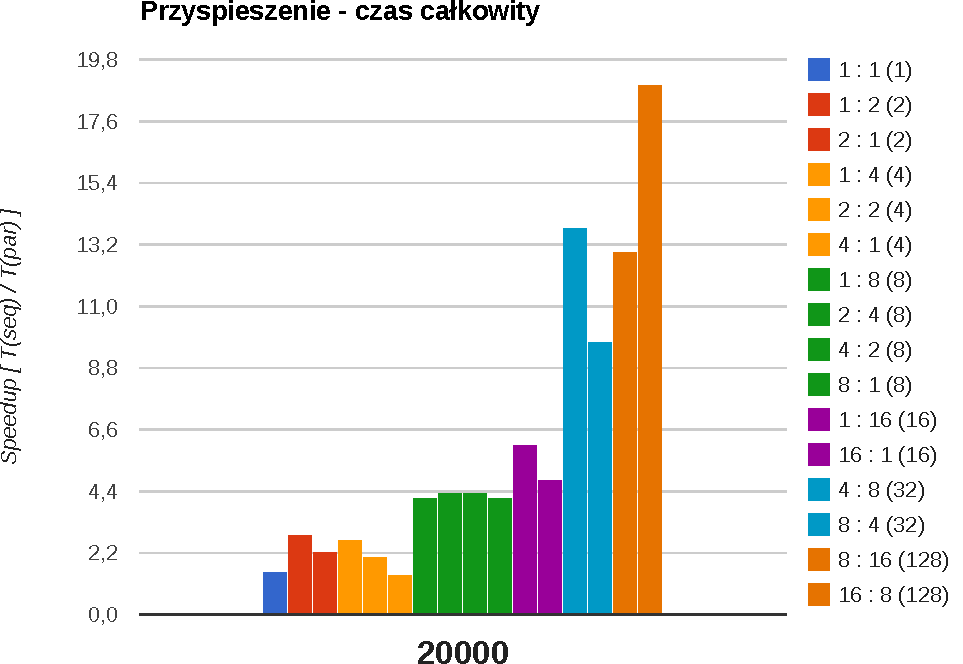
\includegraphics[width=135mm]{report/speedup-20000.pdf} \\ \ \\ \ \\ \ \\

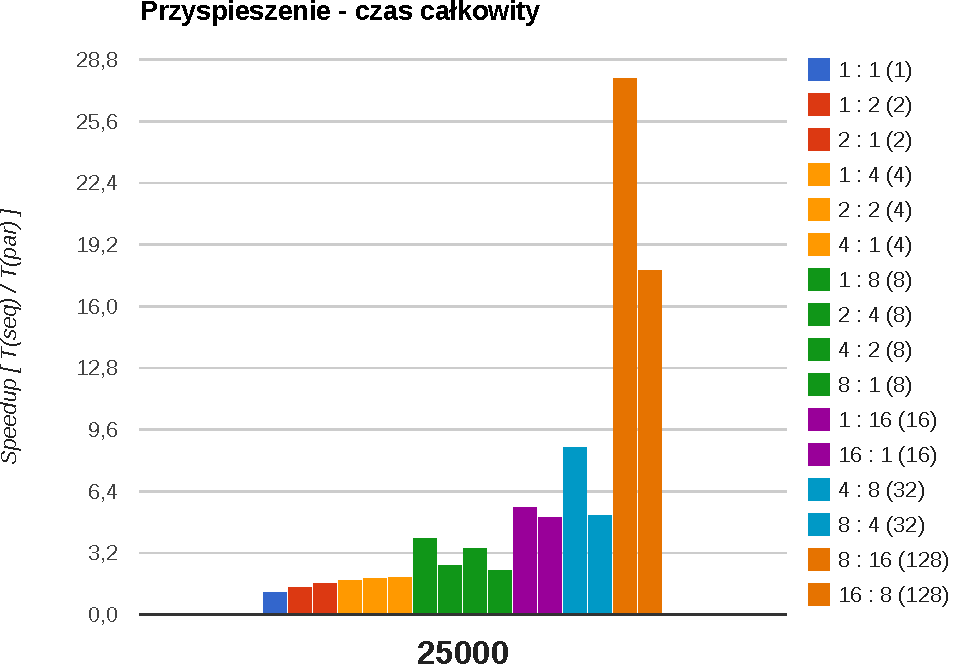
\includegraphics[width=135mm]{report/speedup-25000.pdf} \\ \ \\ \ \\ \ \\

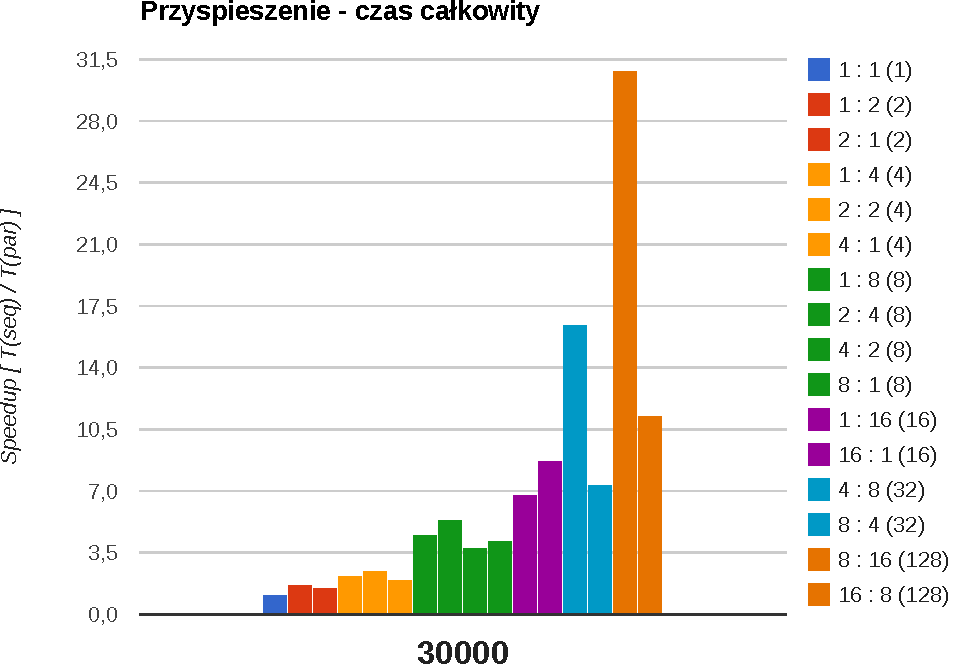
\includegraphics[width=135mm]{report/speedup-30000.pdf} \\ \ \\ \ \\ \ \\

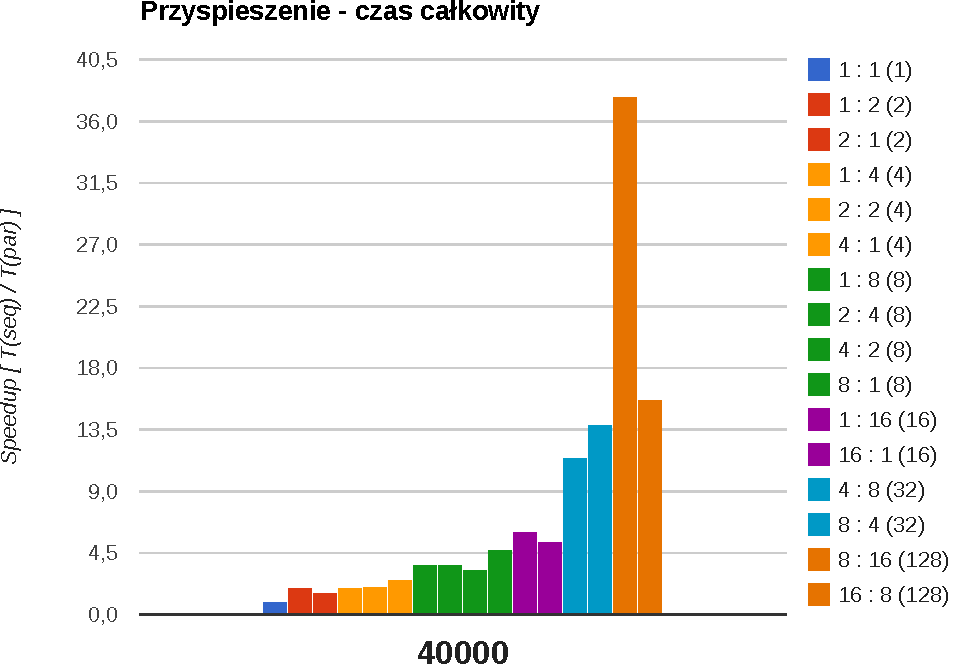
\includegraphics[width=135mm]{report/speedup-40000.pdf} \\ \ \\ \ \\ \ \\

\end{center}


\subsubsection{Speedup obliczeń}

Nieco ciekawsze są wykresy uwzględniające jedynie czas zużyty na obliczenia.
Wyniki są dużo bardziej stabilne i efektywniejsze. Ukazuje to jak dużym
obciążeniem w programie rozproszonym jest synchronizacja. \\ \ \\

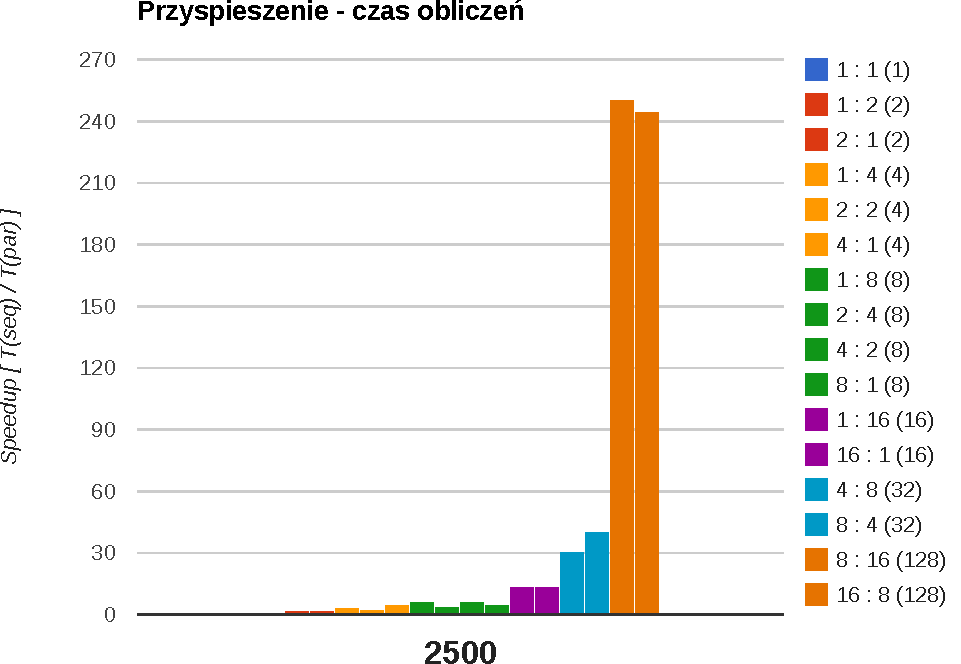
\includegraphics[width=135mm]{report/comp-speedup-2500.pdf} \\ \ \\ \ \\ \ \\

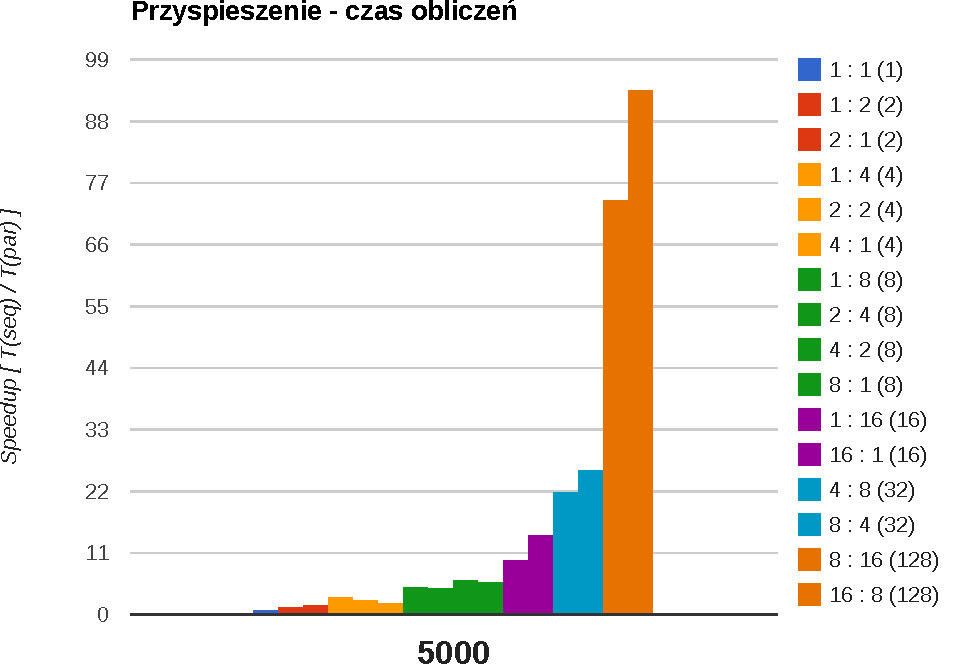
\includegraphics[width=135mm]{report/comp-speedup-5000.pdf} \\ \ \\ \ \\ \ \\

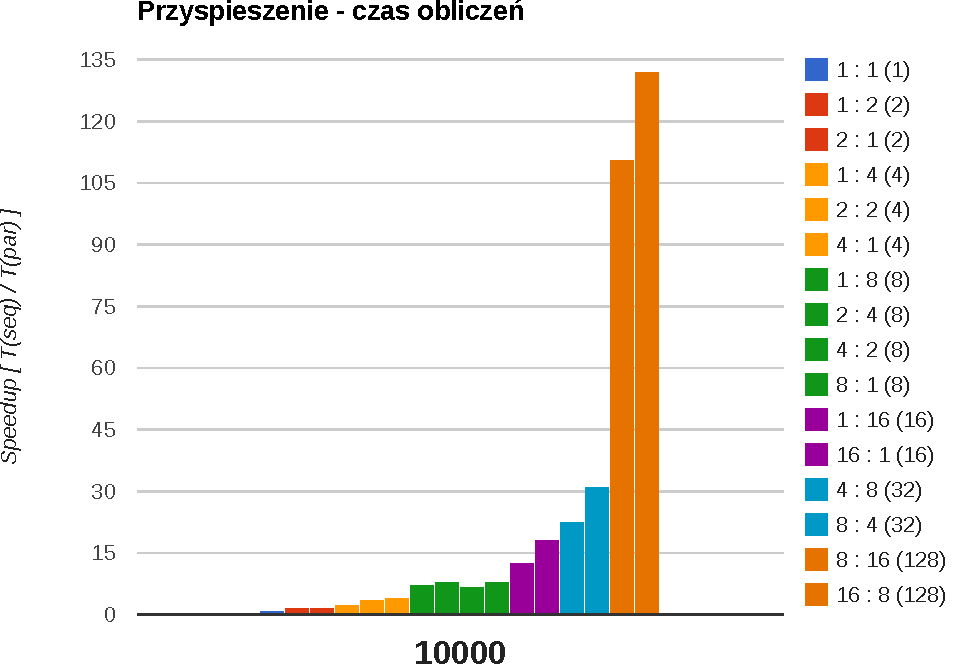
\includegraphics[width=135mm]{report/comp-speedup-10000.pdf} \\ \ \\ \ \\ \ \\

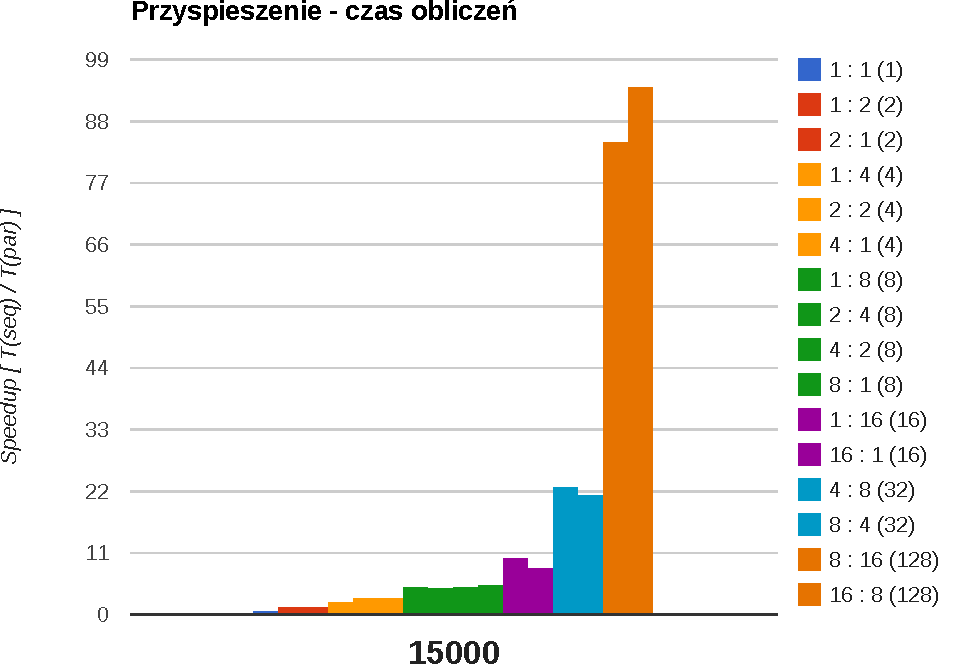
\includegraphics[width=135mm]{report/comp-speedup-15000.pdf} \\ \ \\ \ \\ \ \\

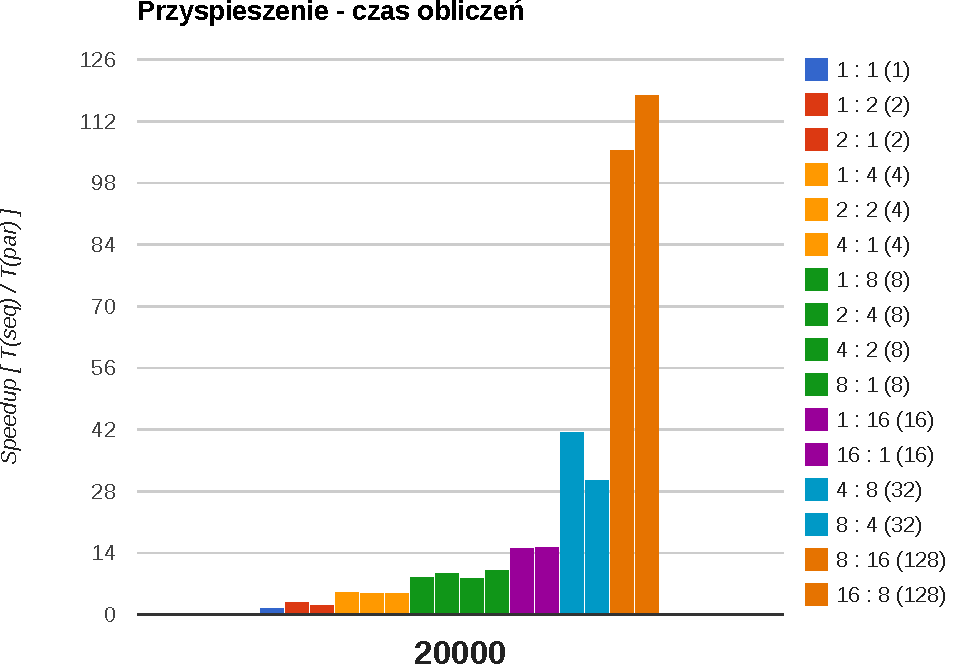
\includegraphics[width=135mm]{report/comp-speedup-20000.pdf} \\ \ \\ \ \\ \ \\

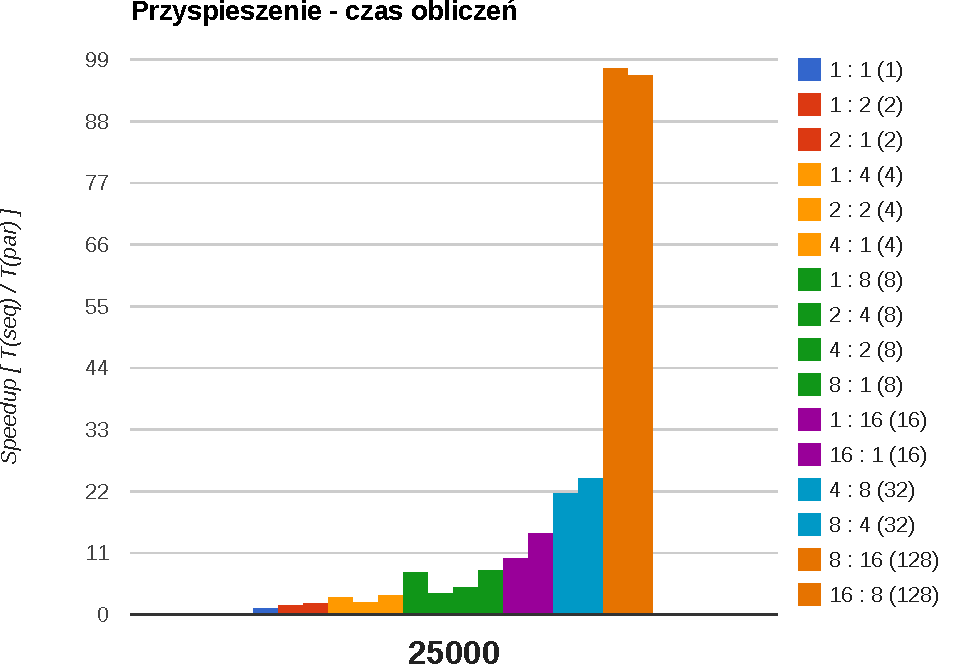
\includegraphics[width=135mm]{report/comp-speedup-25000.pdf} \\ \ \\ \ \\ \ \\

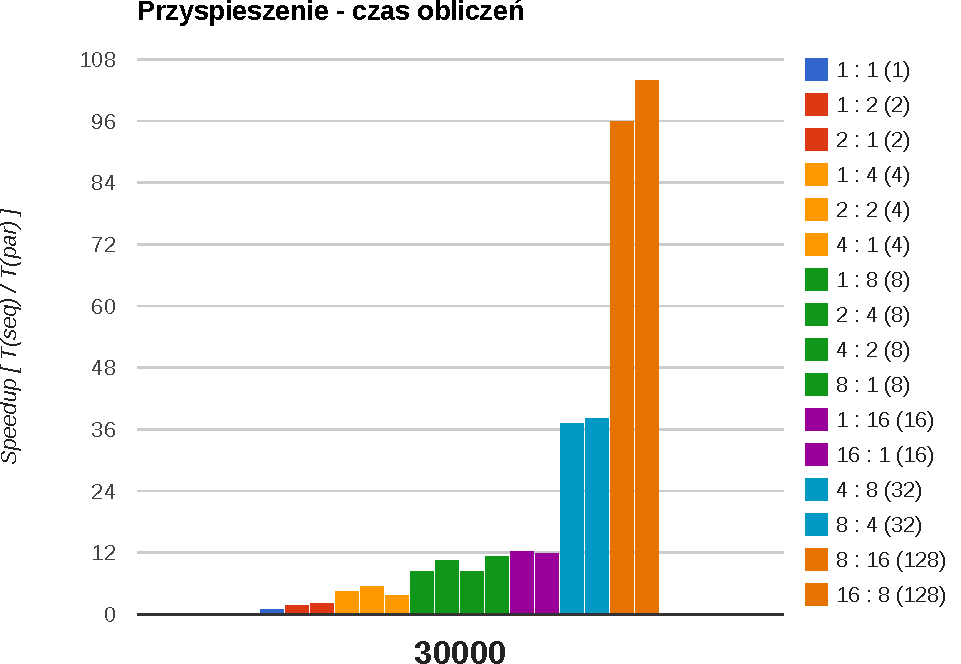
\includegraphics[width=135mm]{report/comp-speedup-30000.pdf} \\ \ \\ \ \\ \ \\

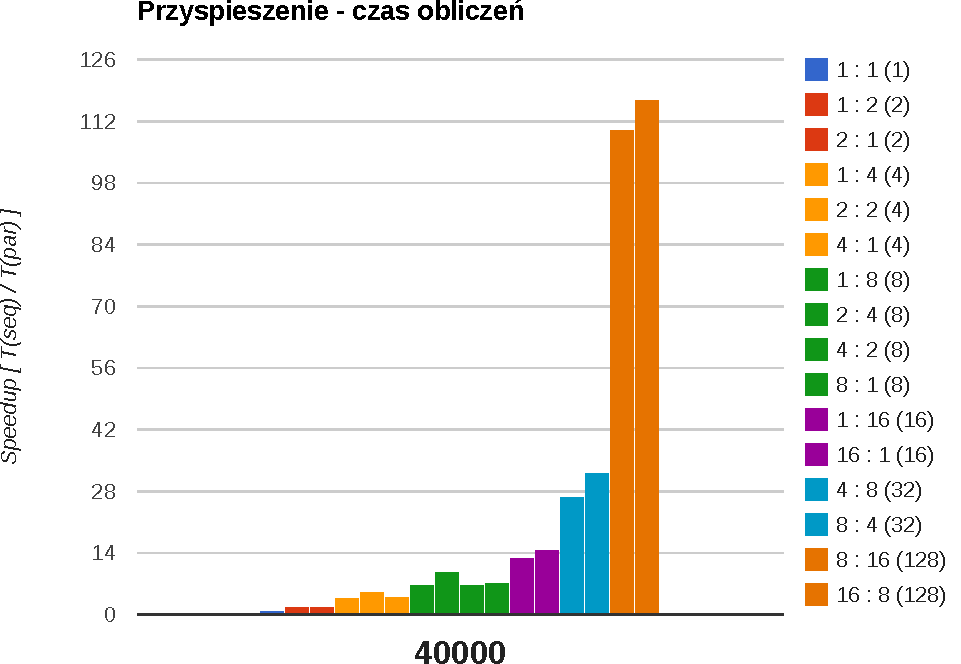
\includegraphics[width=135mm]{report/comp-speedup-40000.pdf} \\ \ \\ \ \\ \ \\


\subsection{Średnia efektywność}

Poniższe wykresy ukazują średnią efektywność dla różnej ilości procesów
biorących udział w teście. Jest ona wyliczona poprzez podzielenie średniego
speedupu z wszystkich testów posiadających tą samą ilość procesów, przez
,,idealny'' speedup, będący funkcją identycznościową od ilosci procesów. \\

W przypadku łącznego czasu widać stopniową degradację jakości zrównoleglenia
wraz ze wzrostem ilości procesów. Jest to spodowane rosnącym kosztem
komunikacji. Ukazuje to kolejny wykres - efektywności obliczeń samych w sobie.
Waha się on nieznacznie w przedziale $\{0.8, 1.0\}$, ale wygląda to jak
zaburzenia spowodowane dużą wariancją czasów, a nie konstrukcją programu. W
szczególności, efektywność wydaje się nie spadać wraz ze wzrostem ilości
procesów, tylko właśnie ,,drgać'' w powyższym przedziale.

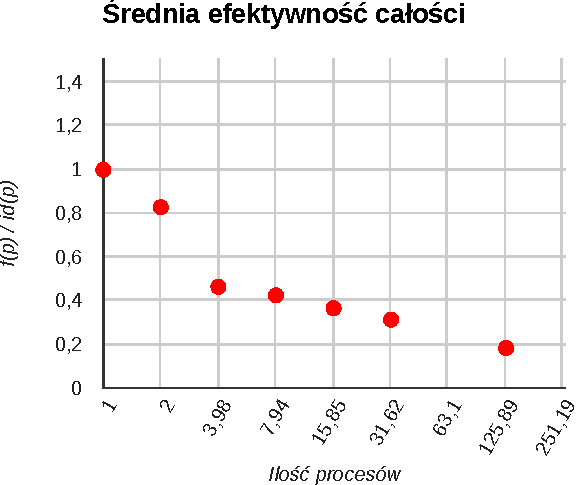
\includegraphics[width=120mm]{report/eff-whole.pdf} \\ \ \\ \ \\ \ \\

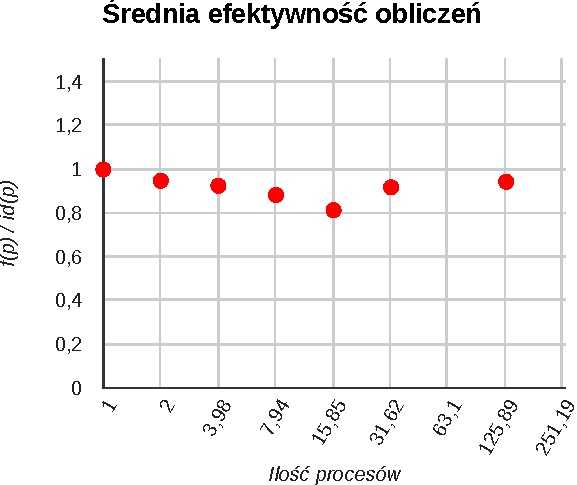
\includegraphics[width=120mm]{report/comp-eff-whole.pdf} \\ \ \\ \ \\ \ \\


\subsection{Efektywność, szczegółowo}

Poniższe wykresy prezentują efektywność dla poszczególnych rozmiarów siatki. W
zasadzie nie mówią wiele więcej niż wykres uśredniony, poza faktem, że przypadek
${N=2500}$ jest niemiarodajny dla większych ilości procesów. Wynika to
najprawdopodobniej z faktu, że czas potrzebny na czynności przygotowawcze do
obliczeń jest wtedy bliski czasowi potrzebne na samo obliczenie i zaciera wynik.

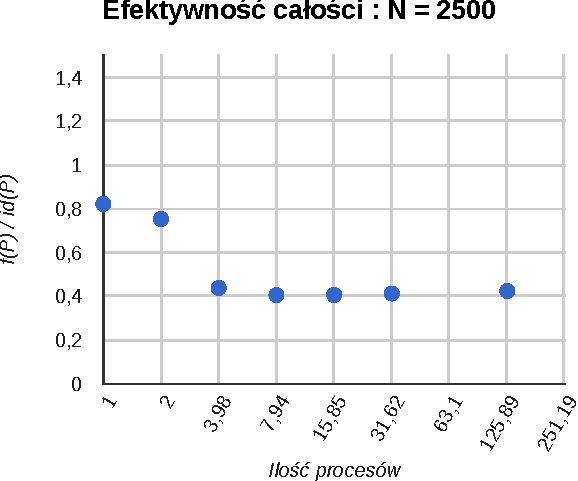
\includegraphics[width=120mm]{report/eff-2500.pdf} \\ \ \\ \ \\ \ \\

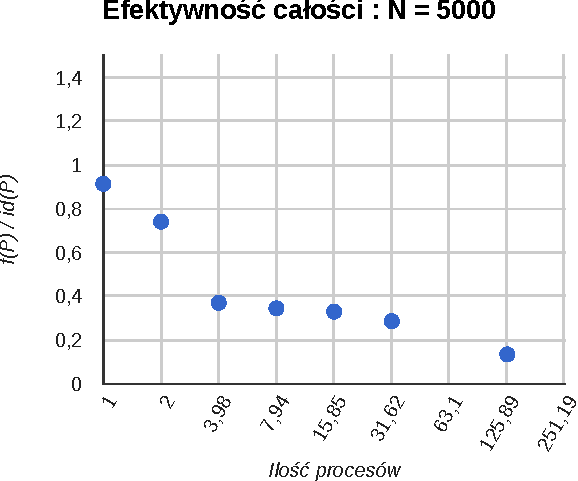
\includegraphics[width=120mm]{report/eff-5000.pdf} \\ \ \\ \ \\ \ \\

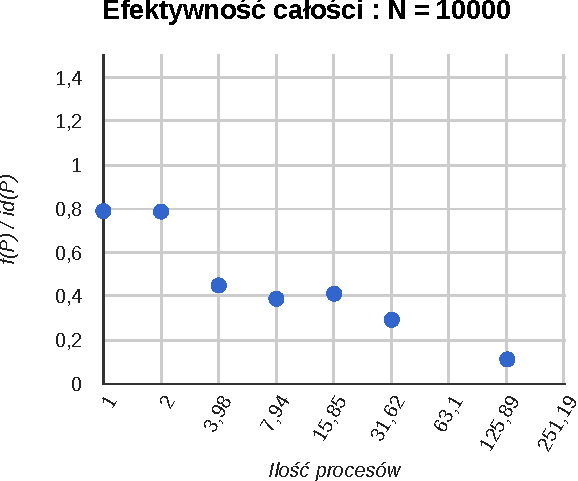
\includegraphics[width=120mm]{report/eff-10000.pdf} \\ \ \\ \ \\ \ \\

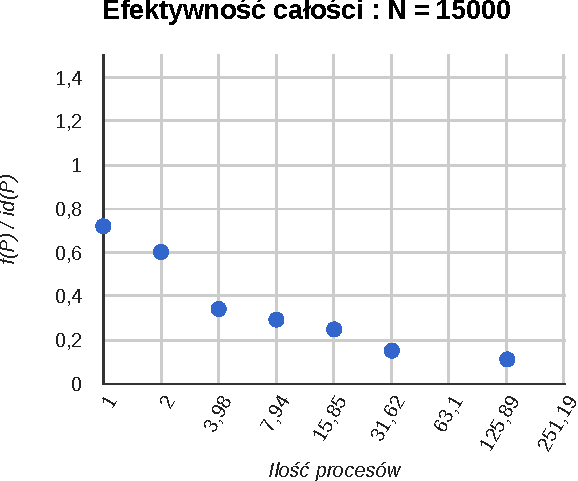
\includegraphics[width=120mm]{report/eff-15000.pdf} \\ \ \\ \ \\ \ \\

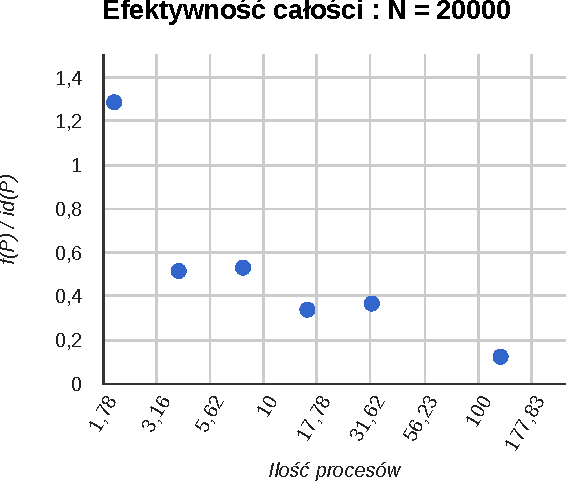
\includegraphics[width=120mm]{report/eff-20000.pdf} \\ \ \\ \ \\ \ \\

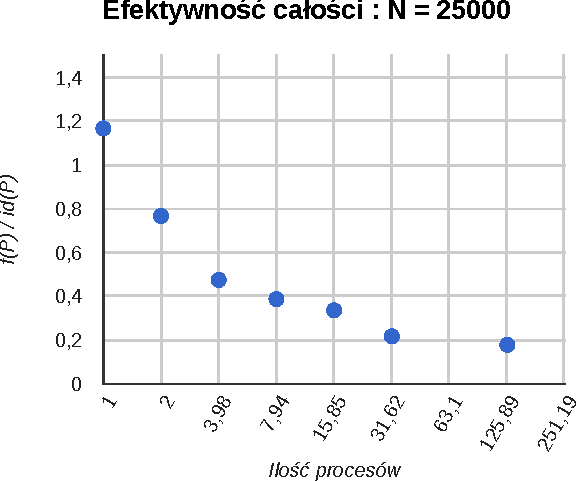
\includegraphics[width=120mm]{report/eff-25000.pdf} \\ \ \\ \ \\ \ \\

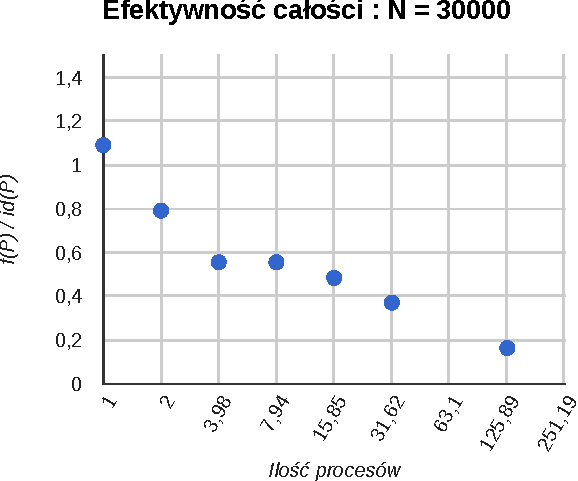
\includegraphics[width=120mm]{report/eff-30000.pdf} \\ \ \\ \ \\ \ \\

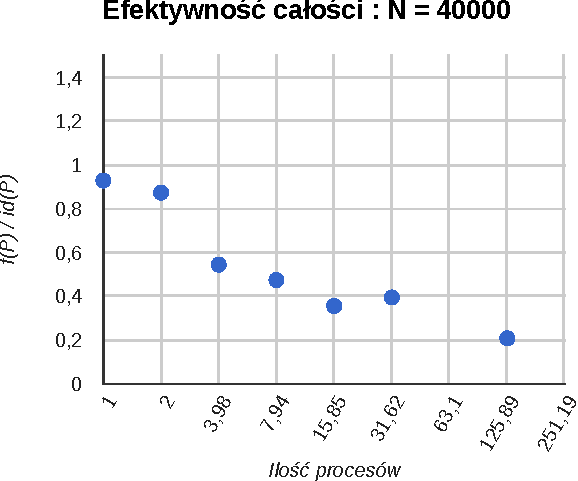
\includegraphics[width=120mm]{report/eff-40000.pdf} \\ \ \\ \ \\ \ \\


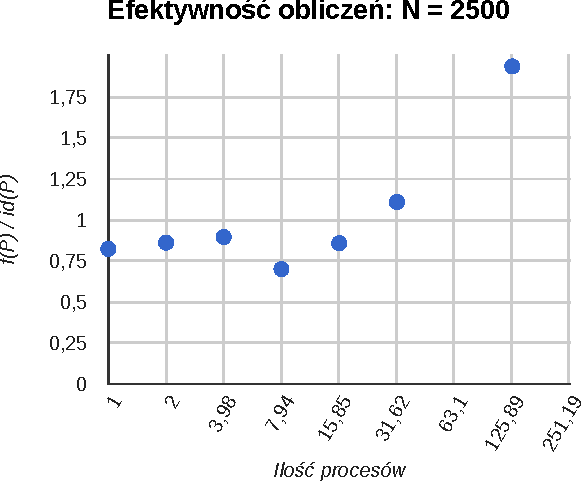
\includegraphics[width=120mm]{report/comp-eff-2500.pdf} \\ \ \\ \ \\ \ \\

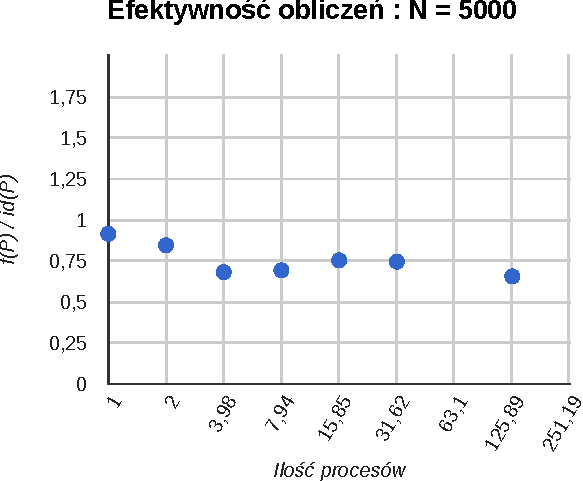
\includegraphics[width=120mm]{report/comp-eff-5000.pdf} \\ \ \\ \ \\ \ \\

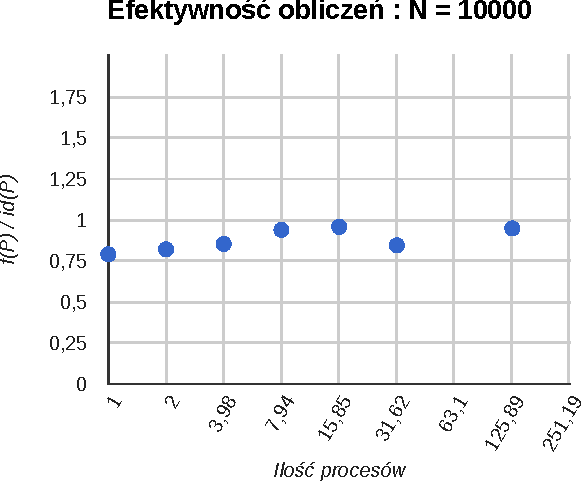
\includegraphics[width=120mm]{report/comp-eff-10000.pdf} \\ \ \\ \ \\ \ \\

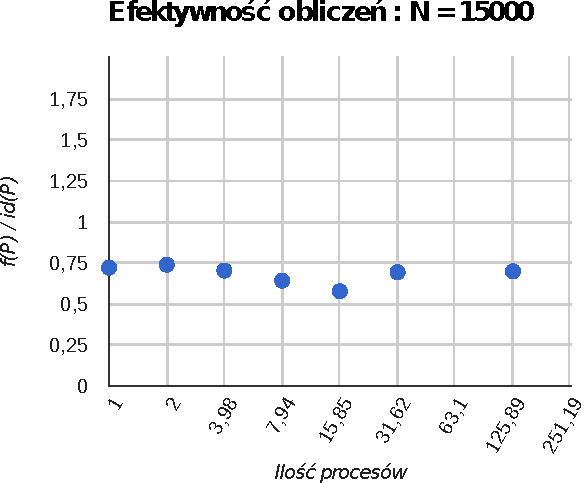
\includegraphics[width=120mm]{report/comp-eff-15000.pdf} \\ \ \\ \ \\ \ \\

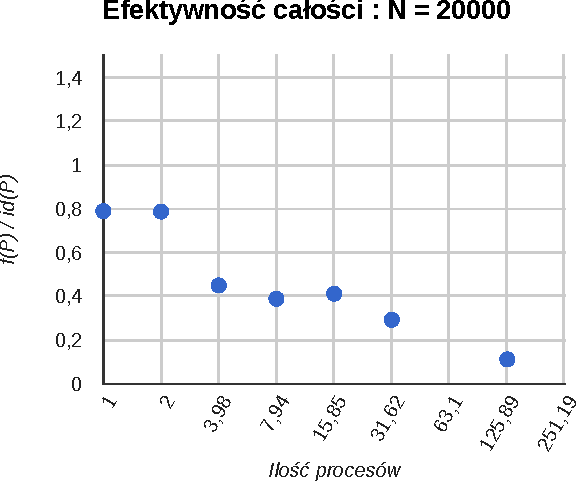
\includegraphics[width=120mm]{report/comp-eff-20000.pdf} \\ \ \\ \ \\ \ \\

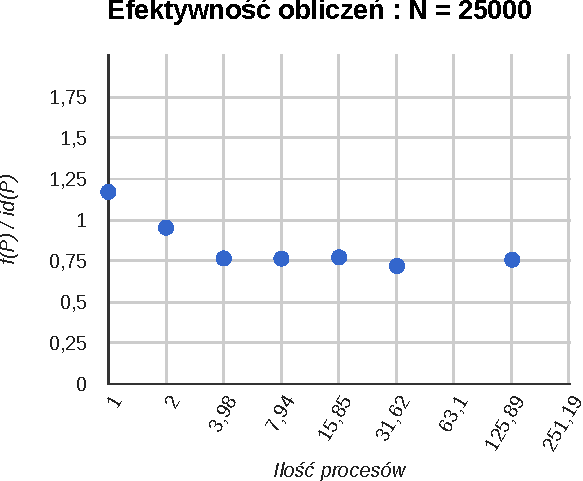
\includegraphics[width=120mm]{report/comp-eff-25000.pdf} \\ \ \\ \ \\ \ \\

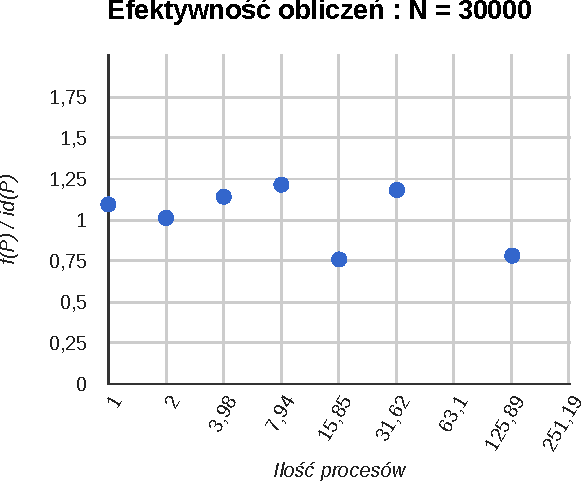
\includegraphics[width=120mm]{report/comp-eff-30000.pdf} \\ \ \\ \ \\ \ \\

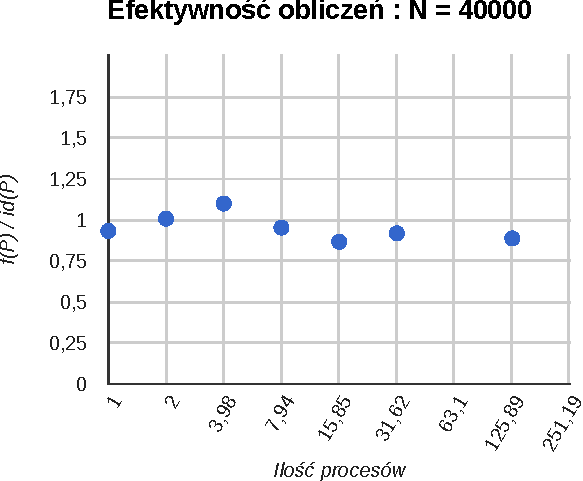
\includegraphics[width=120mm]{report/comp-eff-40000.pdf} \\ \ \\ \ \\ \ \\


\subsubsection{Performance breakdown}

Na koniec pozostał performance breakdown, czyli podział czasu ze względu na typ
wykonywanych czynności. Poniższe wykresu ukazują podział całkowitego czasu
wykonania na obliczenie i komunikację. \\

Jak widać komunikacja zajmuje dużą, a od pewnego momentu wręcz większą część
czasu. Udział ten wydaje się być słabo skorelowany z rozmiarem siatki, za to
mocno z ilością procesów. \\

Ponadto, konfiguracje z większą ilością rdzeni niż maszyn ponownie wydają się
mieć pewną przewagę pod względem części czasu przeznaczonego na obliczenia. \\
\\


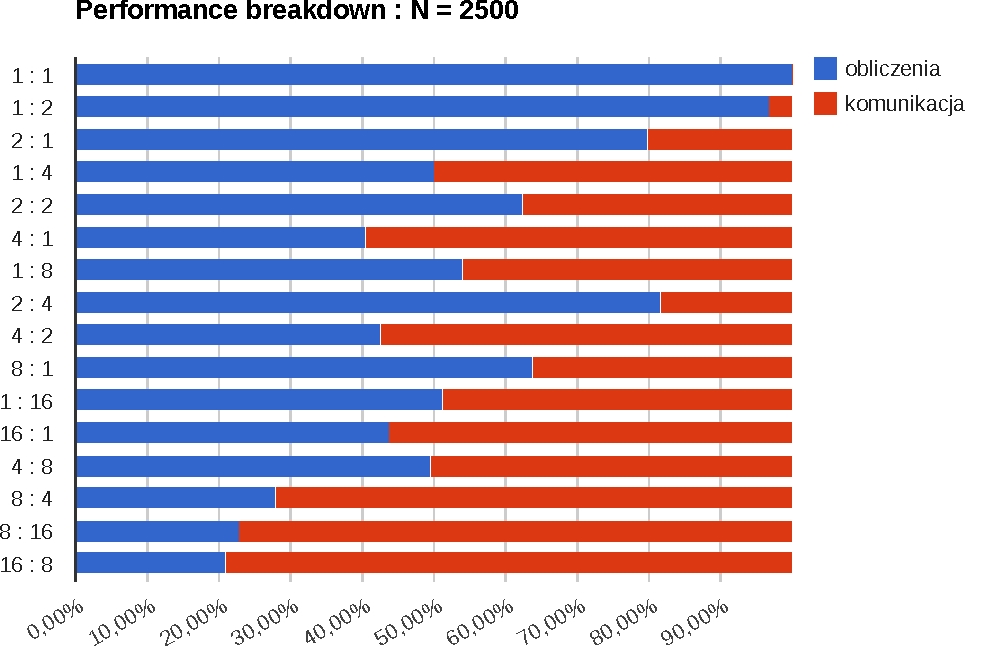
\includegraphics[width=135mm]{report/breakdown-2500.pdf} \\ \ \\ \ \\ \ \\

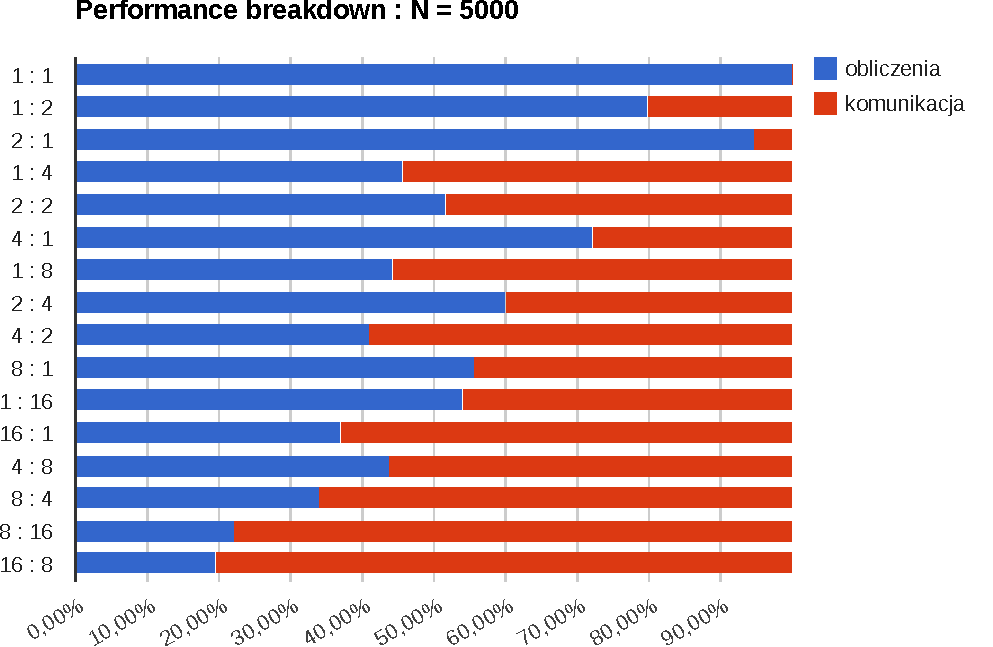
\includegraphics[width=135mm]{report/breakdown-5000.pdf} \\ \ \\ \ \\ \ \\

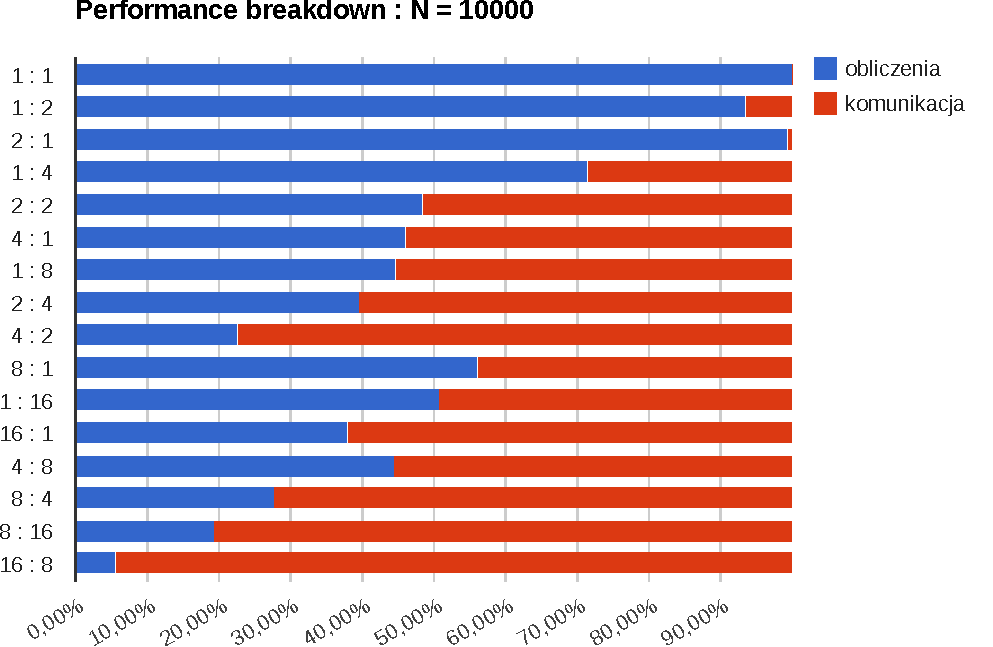
\includegraphics[width=135mm]{report/breakdown-10000.pdf} \\ \ \\ \ \\ \ \\

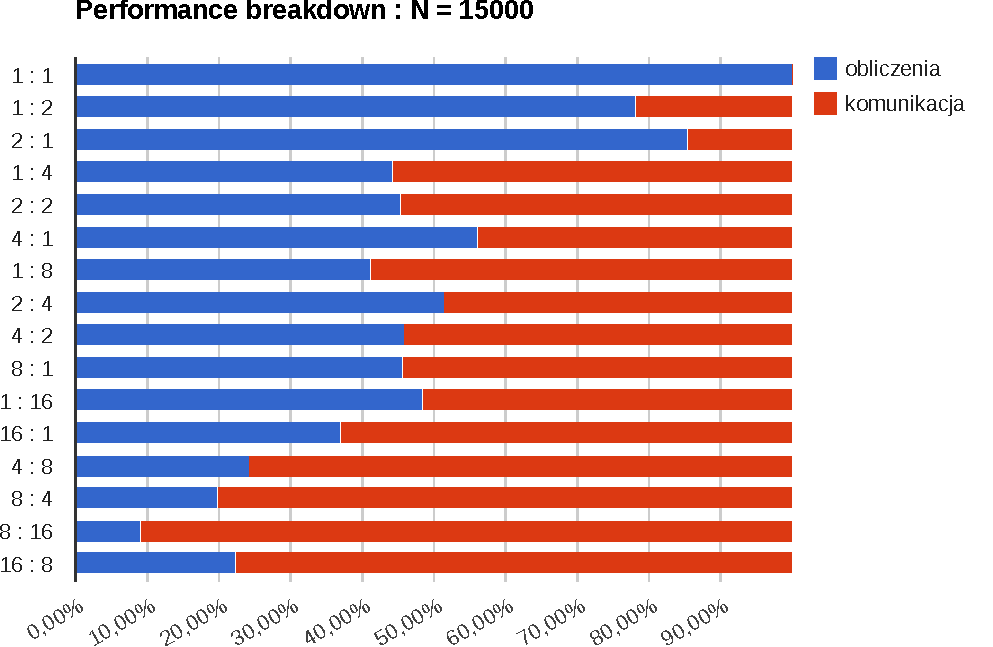
\includegraphics[width=135mm]{report/breakdown-15000.pdf} \\ \ \\ \ \\ \ \\

\includegraphics[width=135mm]{report/breakdown-20000.pdf} \\ \ \\ \ \\ \ \\

\includegraphics[width=135mm]{report/breakdown-25000.pdf} \\ \ \\ \ \\ \ \\

\includegraphics[width=135mm]{report/breakdown-30000.pdf} \\ \ \\ \ \\ \ \\

\includegraphics[width=135mm]{report/breakdown-40000.pdf} \\ \ \\ \ \\ \ \\


\section{Podsumowanie}

Program współbieżny skaluje się, chociaż nie tak dobrze jak można by tego
oczekiwać / chcieć. Wina, wyraźnie leży po stronie komunikacji i synchronizacji
między procesami. Można by spróbować to naprawić zmieniając sposób dzielenia
siatki między procesy (tak, by zmniejszyć ilość przesyłanych danych) oraz
zwiększając asynchroniczność komunikacji (np. podczas ustalania maksymalnej
różnicy wartości punktów). \\

Ponadto, warto by przeanalizować program pod względem trafień w pamięć
podręczną. Być może niewielka zmiana struktur danych bądź kolejności wykonywania
obliczeń mogła by spowodować znaczne przyspieszenie.

%%% End document
\end{document}
